% SC2001 — Chapter 4: Divide and Conquer
% No \documentclass — included by main.tex
\chapter{Divide and Conquer}
\label{ch:divide-conquer}

\begin{quote}
\emph{``Divide et impera.''} --- The oldest strategy in warfare is also one of the most powerful in algorithm design: break a hard problem into smaller copies of itself, solve them recursively, and combine.
\end{quote}

\noindent\textbf{Prerequisites:} Recurrences and asymptotics (Ch.~2), induction (Ch.~1), basic probability --- see Micro-primer~\S\ref{sec:prob-primer} for indicators and linearity used in QuickSort.

\section*{Learning Outcomes}
After this chapter you will be able to:
\begin{enumerate}[label=(L\arabic*)]
    \item state the D\&C paradigm and write recurrences for D\&C algorithms;
    \item prove correctness and $\Theta(n\log n)$ complexity of MergeSort;
    \item analyse deterministic vs.\ randomised QuickSort (worst case vs.\ expected $O(n\log n)$ via indicator variables);
    \item prove the strip sparsity lemma for the closest-pair problem;
    \item derive Strassen's 7-multiplication recurrence and its $O(n^{\log_2 7})$ bound.
\end{enumerate}

% ============================================================
\section{The Divide-and-Conquer Paradigm}
\label{sec:dc-paradigm}

A D\&C algorithm for input size $n$ does three steps:
\begin{enumerate}[label=\arabic*.]
    \item \textbf{Divide} the instance into $a\ge 1$ subinstances each of size $\lceil n/b\rceil$ or $\lfloor n/b\rfloor$ ($b>1$).
    \item \textbf{Conquer} by solving subinstances recursively (base case $n\le n_0$ solved directly).
    \item \textbf{Combine} sub-solutions into a solution for the original instance at cost $f(n)$.
\end{enumerate}
\begin{figure}[h!]
\centering
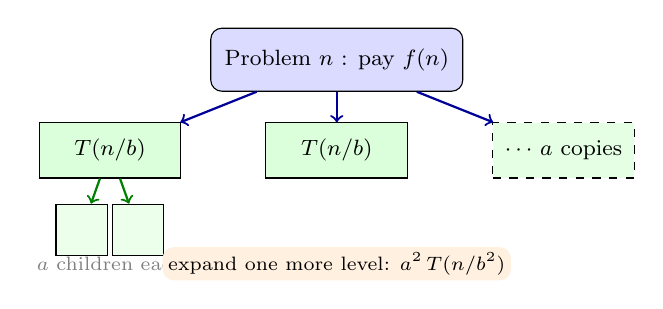
\begin{tikzpicture}[scale=0.72, every node/.style={font=\footnotesize}]
  \node[draw,rounded corners,fill=blue!14,minimum width=3.2cm,minimum height=0.8cm] (rt) at (4,2.2) {Problem $n$ : pay $f(n)$};
  \node[draw,fill=green!14,minimum width=1.8cm,minimum height=0.7cm] (c1) at (0,0.6) {$T(n/b)$};
  \node[draw,fill=green!14,minimum width=1.8cm,minimum height=0.7cm] (c2) at (4,0.6) {$T(n/b)$};
  \node[draw,fill=green!10,minimum width=1.8cm,minimum height=0.7cm,dashed] (c3) at (8,0.6) {$\cdots$ $a$ copies};
  \draw[->,thick,blue!60!black] (rt) -- (c1); \draw[->,thick,blue!60!black] (rt) -- (c2); \draw[->,thick,blue!60!black] (rt) -- (c3);
  \node[draw,fill=green!8,minimum size=0.65cm] (g1) at (-0.5,-0.8) {};\node[draw,fill=green!8,minimum size=0.65cm] (g2) at (0.5,-0.8) {};
  \draw[->,thick,green!50!black] (c1) -- (g1); \draw[->,thick,green!50!black] (c1) -- (g2);
  \node[font=\scriptsize,color=gray] at (0,-1.4) {$a$ children each};
  \node[font=\scriptsize,fill=orange!12,rounded corners,inner sep=2pt] at (4,-1.4) {expand one more level: $a^2\,T(n/b^2)$};
\end{tikzpicture}
\caption{Two-level D\&C tree: root combine cost $f(n)$ plus $a$ subproblems $T(n/b)$. Summing levels gives $T(n)=a\,T(n/b)+f(n)$, $T(1)=\Theta(1)$.}
\label{fig:dc-tree}
\end{figure}
Hence
\begin{equation}
T(n)=a\,T(n/b)+f(n),\qquad T(1)=\Theta(1). \label{eq:dc-rec}
\end{equation}
The Master Theorem (Ch.~3, Thm.~\ref{thm:master}) classifies \eqref{eq:dc-rec}: if $f(n)=O(n^{\log_b a-\epsilon})$ then $T(n)=\Theta(n^{\log_b a})$; if $f(n)=\Theta(n^{\log_b a})$ then $T(n)=\Theta(n^{\log_b a}\log n)$; if $f(n)=\Omega(n^{\log_b a+\epsilon})$ and regular then $T(n)=\Theta(f(n))$.
D\&C wins when the combine cost is cheap relative to shrinkage; the next sections make this concrete.

% ============================================================
\section{MergeSort}
\label{sec:mergesort}

\texttt{MergeSort}$(A[p..r])$: if $p<r$, let $q=\lfloor(p+r)/2\rfloor$, recursively sort $A[p..q]$ and $A[q+1..r]$, then \texttt{Merge} the two sorted halves in $\Theta(n)$ time using an auxiliary array.

\begin{theorem}[Correctness of MergeSort]
\texttt{MergeSort} returns a permutation of the input sorted in nondecreasing order.
\end{theorem}
\begin{proof}
Induction on $n=r-p+1$. Base $n=1$ trivially sorted. Assume holds for all sizes $<n$. Both halves are sorted by IH. \texttt{Merge} repeatedly takes the smaller leading element, so output is sorted and contains exactly $A[p..r]$. By induction the claim holds.
\end{proof}

\texttt{Merge} scans each element once, so $f(n)=\Theta(n)$. Thus $T(n)=2T(n/2)+\Theta(n)$, $T(1)=\Theta(1)$. Here $a=2$, $b=2$, $\log_b a=1$, $f(n)=\Theta(n)=\Theta(n^{\log_b a})$, so Master case~2 gives $T(n)=\Theta(n\log n)$. This is asymptotically optimal for comparison sorting (Ch.~8). MergeSort guarantees $\Theta(n\log n)$ worst-case but needs $\Theta(n)$ extra space.

% ============================================================
\subsection*{Micro-primer: Indicator Variables and Linearity of Expectation}
\label{sec:prob-primer}
For an event $E$ the \emph{indicator} $X=\mathbf{1}[E]$ is $1$ if $E$ occurs else $0$; then $\mathbb{E}[X]=\Pr[E]$ because $\mathbb{E}[X]=1\cdot\Pr[E]+0\cdot\Pr[\bar E]$. \emph{Linearity:} for any $X_i$ (dependent or not), $\mathbb{E}[\sum_i X_i]=\sum_i\mathbb{E}[X_i]$; expectation of a sum is the sum of expectations, by definition $\sum_x x\Pr[X=x]$.
\emph{Example (2 coins):} toss fair coins with $X_1=\mathbf{1}[\text{coin 1 is H}]$, $X_2=\mathbf{1}[\text{coin 2 is H}]$; $\mathbb{E}[X_i]=1/2$, $\mathbb{E}[X_1+X_2]=1$ even though $X_1,X_2$ are independent, and $\mathbb{E}[2X_1]=1$ by scaling. For QuickSort we write total comparisons $X=\sum_{i<j}X_{ij}$ with each $X_{ij}\in\{0,1\}$ and use $\mathbb{E}[X]=\sum_{i<j}\Pr[X_{ij}=1]$ without needing independence.

% ============================================================
\section{QuickSort}
\label{sec:quicksort}

\texttt{Partition}$(A,p,r)$ picks pivot $x=A[r]$, maintains $i$ with $A[p..i]\le x$ and $A[i+1..j-1]>x$, scanning $j$ from $p$ to $r-1$ and swapping when $A[j]\le x$. Finally swap $A[i+1]$ with $A[r]$; return $q=i+1$. Cost is $\Theta(n)$.

\begin{figure}[h!]
\centering
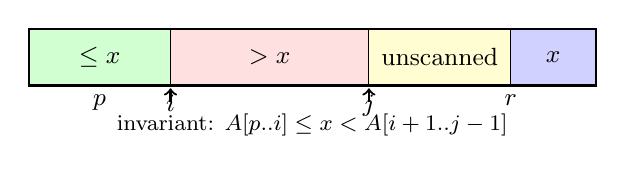
\begin{tikzpicture}[scale=0.72, every node/.style={font=\small}]
  \fill[green!18] (0,0) rectangle (2.5,1);
  \fill[red!12] (2.5,0) rectangle (6,1);
  \fill[yellow!18] (6,0) rectangle (8.5,1);
  \fill[blue!18] (8.5,0) rectangle (10,1);
  \draw[thick] (0,0) rectangle (10,1);
  \draw (2.5,0) -- (2.5,1); \draw (6,0) -- (6,1); \draw (8.5,0) -- (8.5,1);
  \node at (1.25,0.5) {$\le x$}; \node at (4.25,0.5) {$>x$};
  \node at (7.25,0.5) {unscanned}; \node at (9.25,0.5) {$x$};
  \node[below] at (1.25,0) {$p$}; \node[below] at (2.5,0) {$i$};
  \node[below] at (6,0) {$j$}; \node[below] at (8.5,0) {$r$};
  \draw[->,thick] (2.5,-0.3) -- (2.5,-0.05); \draw[->,thick] (6,-0.3) -- (6,-0.05);
  \node[font=\footnotesize] at (5,-0.7) {invariant: $A[p..i]\le x < A[i+1..j-1]$};
\end{tikzpicture}
\caption{Lomuto partition invariant.}
\label{fig:qs-partition}
\end{figure}

\texttt{QuickSort}$(A,p,r)$: if $p<r$, $q\leftarrow$\texttt{Partition}$(A,p,r)$, recurse on $A[p..q-1]$ and $A[q+1..r]$.

\paragraph{Deterministic worst case.} If pivot is always smallest or largest (e.g., sorted input with $A[r]$ as pivot), partitions are $0$ and $n-1$: $T(n)=T(n-1)+\Theta(n)=\Theta(\sum_{k=1}^{n}k)=\Theta(n^2)$.\newline Balanced partitions ($n/4$--$3n/4$) give $T(n)\le 2T(3n/4)+\Theta(n)=\Theta(n\log n)$, but the adversary can force $\Theta(n^2)$.

\paragraph{Randomised QuickSort.} Choose pivot uniformly at random from $A[p..r]$ (or randomly permute first). Let $z_1<\cdots<z_n$ be sorted values and $X_{ij}=1$ if $z_i$ and $z_j$ are ever compared (one is chosen as pivot while both in same call), else $0$. Total comparisons $X=\sum_{i<j}X_{ij}$.

\begin{figure}[h!]
\centering
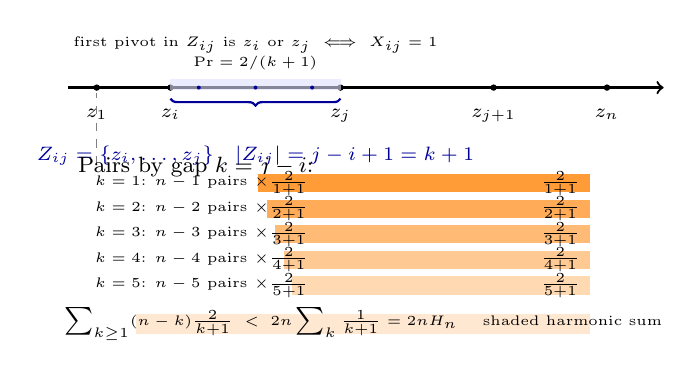
\begin{tikzpicture}[scale=0.72, every node/.style={font=\scriptsize}]
  \draw[thick,->] (0,1.4) -- (10.5,1.4);
  \foreach \x/\lab in {0.5/$z_1$,1.8/$z_i$,4.8/$z_j$,7.5/$z_{j+1}$,9.5/$z_n$} {\fill (\x,1.4) circle (1.6pt); \node[below] at (\x,1.2) {\lab};}
  \draw[decorate,decoration={brace,mirror,raise=4pt},thick,blue!60!black] (1.8,1.4) -- (4.8,1.4);
  \node[blue!60!black,below] at (3.3,0.55) {$Z_{ij}=\{z_i,\dots,z_j\}$ \; $|Z_{ij}|=j-i+1=k+1$};
  \fill[blue!12,opacity=0.6] (1.8,1.35) rectangle (4.8,1.55);
  \foreach \x in {2.3,3.3,4.3} {\fill[blue!60!black] (\x,1.4) circle (1pt);}
  \node[font=\tiny,align=center] at (3.3,2.0) {first pivot in $Z_{ij}$ is $z_i$ or $z_j$ $\iff$ $X_{ij}=1$ \\ $\Pr=2/(k+1)$};
  \draw[dashed,gray] (0.5,0.05) -- (0.5,1.3);
  \node[font=\footnotesize,anchor=west] at (0,0) {Pairs by gap $k=j-i$:};
  \foreach \k in {1,2,3,4,5} {
    \pgfmathsetmacro{\y}{-0.45*\k}
    \pgfmathsetmacro{\op}{max(15, 90-12*\k)}
    \fill[orange!\op] (3.2+\k*0.15,\y) rectangle (9.2,\y+0.32);
    \node[anchor=west,font=\tiny] at (0.3,\y+0.16) {$k=\k$: $n-\k$ pairs $\times\frac{2}{\k+1}$};
    \node[anchor=east,font=\tiny] at (9.2,\y+0.16) {$\frac{2}{\k+1}$};
  }
  \fill[orange!18] (1.2,-2.6) rectangle (9.2,-2.95);
  \node[font=\tiny,align=left] at (5.2,-2.77) {$\sum_{k\ge1}(n-k)\frac{2}{k+1}\;<\;2n\sum_{k}\frac1{k+1}=2nH_n$ \quad shaded harmonic sum};
\end{tikzpicture}
\caption{Indicator view: interval $Z_{ij}$ on sorted line (blue) and triangle of $\frac{2}{k+1}$ terms by gap $k$; shading $=$ harmonic sum $H_n$.}
\label{fig:qs-indicator}
\end{figure}
For $i<j$, $z_i$ and $z_j$ are compared iff among $Z_{ij}$ the first pivot chosen is $z_i$ or $z_j$. All $|Z_{ij}|=j-i+1$ are equally likely first, so $\Pr[X_{ij}=1]=2/(j-i+1)$ and $\mathbb{E}[X_{ij}]=2/(j-i+1)$. By linearity (Micro-primer),
\[\mathbb{E}[X]=\sum_{i<j}\frac{2}{j-i+1}=\sum_{i=1}^{n}\sum_{k=1}^{n-i}\frac{2}{k+1}<2\sum_{i}H_n=O(n\log n),\]
more precisely $\mathbb{E}[X]=2(n+1)H_n-4n\sim2n\ln n$. Each comparison is $O(1)$, so $\mathbb{E}[T(n)]=O(n\log n)$. Randomisation removes the adversary: \emph{every} input has expected $O(n\log n)$.

% ============================================================
\section{Closest Pair of Points}
\label{sec:closest-pair}

Given $P=\{p_1,\dots,p_n\}\subset\mathbb{R}^2$, find $\min_{i\ne j}\|p_i-p_j\|_2$. Brute force is $\Theta(n^2)$. D\&C: sort by $x$, split by median $x=m$ into $P_L,P_R$, recursively find $\delta_L,\delta_R$, set $\delta=\min(\delta_L,\delta_R)$, then check pairs straddling the line within vertical strip $|x-m|<\delta$.

\begin{figure}[h!]
\centering
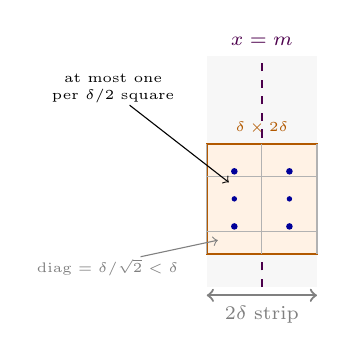
\begin{tikzpicture}[scale=0.70, every node/.style={font=\scriptsize}]
  \fill[gray!6] (3,0) rectangle (5,4.2);
  \draw[dashed,thick,violet!60!black] (4,0) -- (4,4.2) node[above,violet!60!black] {$x=m$};
  \draw[<->,thick,gray] (3,-0.15) -- (5,-0.15) node[midway,below] {$2\delta$ strip};
  \draw[thick,orange!70!black,fill=orange!10] (3,0.6) rectangle (5,2.6);
  \node[orange!70!black,font=\tiny,above] at (4,2.6) {$\delta\times2\delta$};
  \draw[step=1cm,gray!60,thin] (3,0.6) grid (5,2.6);
  \foreach \x in {3.5,4.5} \foreach \y in {1.1,2.1} {\fill[blue!60!black] (\x,\y) circle (1.7pt);}
  \foreach \x in {3.5,4.5} {\fill[blue!60!black] (\x,1.6) circle (1.4pt);}
  \node[font=\tiny,align=center,fill=white,rounded corners,inner sep=1pt] at (1.3,3.6) {at most one\\per $\delta/2$ square};
  \draw[->,thin] (1.6,3.3) -- (3.4,1.9);
  \node[font=\tiny,gray] at (1.2,0.35) {diag $=\delta/\sqrt2<\delta$};
  \draw[->,thin,gray] (1.8,0.55) -- (3.2,0.85);
\end{tikzpicture}
\caption{Strip sparsity: any $\delta\times2\delta$ rectangle in the $2\delta$ strip splits into $8$ squares of side $\delta/2$; diagonal $\delta/\sqrt2<\delta$, so each square holds at most one point --- at most $7$ successors need be checked.}
\label{fig:strip}
\end{figure}

\begin{lemma}[Strip sparsity]
Any $\delta\times2\delta$ rectangle in the strip contains at most $8$ points of $P$ (hence at most $7$ successors need be checked; tighter packing gives $6$).
\end{lemma}
\begin{proof}
Partition the rectangle into $8$ squares of side $\delta/2$ ($2$ columns $\times 4$ rows). Diagonal is $\delta/\sqrt2<\delta$. If two points lay in the same square their distance would be $<\delta$, contradicting that distances within $P_L$ and $P_R$ are $\ge\delta$. So at most one per square.
\end{proof}

Consequently, for each point in the strip sorted by $y$, only the next $7$ points need be checked. The strip scan is $O(n)$ after $O(n\log n)$ presorting (or $O(n)$ with presorted arrays passed down). Recurrence: $T(n)=2T(n/2)+O(n)\Rightarrow T(n)=O(n\log n)$. This beats $\Theta(n^2)$ and is optimal in the algebraic decision-tree model. In practice the $y$-order is maintained by passing the $y$-sorted array through recursion.

\begin{remark}
The closest-pair recurrence is identical in form to MergeSort's; the difficulty is entirely in the combine step. The sparsity lemma is what keeps $f(n)=O(n)$.
\end{remark}

% ============================================================
\section{Strassen's Matrix Multiplication}
\label{sec:strassen}

Naive $n\times n$ multiplication costs $\Theta(n^3)$.
Partition $A=[A_{11}\,A_{12};\,A_{21}\,A_{22}]$,
$B=[B_{11}\,B_{12};\,B_{21}\,B_{22}]$,
$C=AB$ similarly, each block $n/2\times n/2$.
Standard block multiplication needs $8$ half-size products.
Strassen (1969) uses $7$, like Karatsuba's trick:
$ab$ normally needs $4$ products
$(a_1b_1,a_1b_0,$ $a_0b_1,a_0b_0)$ but
$(a_1+a_0)(b_1+b_0)-a_1b_1-a_0b_0$ recovers the cross terms with $3$;
Strassen does the same for $2\times2$ blocks with $7$ products
$M_k$ (each a sum/difference of blocks).

\begin{align*}
M_1&=(A_{11}+A_{22})(B_{11}+B_{22}) & M_5&=(A_{11}+A_{12})B_{22}\\
M_2&=(A_{21}+A_{22})B_{11}           & M_6&=(A_{21}-A_{11})(B_{11}+B_{12})\\
M_3&=A_{11}(B_{12}-B_{22})           & M_7&=(A_{12}-A_{22})(B_{21}+B_{22})\\
M_4&=A_{22}(B_{21}-B_{11}) &&
\end{align*}
Then $C_{11}=M_1+M_4-M_5+M_7$, $C_{12}=M_3+M_5$, $C_{21}=M_2+M_4$, $C_{22}=M_1-M_2+M_3+M_6$. Each $M_k$ is one $n/2\times n/2$ product; the $18$ additions cost $\Theta(n^2)$.

\begin{figure}[h!]
\centering
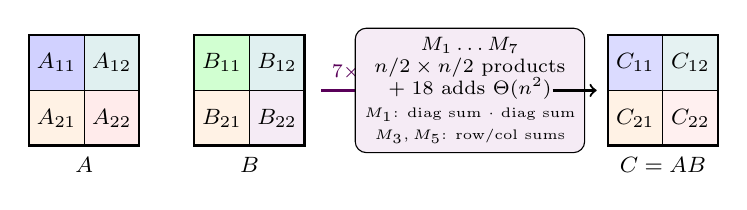
\begin{tikzpicture}[scale=0.70, every node/.style={font=\footnotesize}]
  \fill[blue!10] (0,0) rectangle (2,2);
  \fill[blue!18] (0,1) rectangle (1,2);
  \fill[teal!12] (1,1) rectangle (2,2);
  \fill[orange!10] (0,0) rectangle (1,1);
  \fill[red!8] (1,0) rectangle (2,1);
  \draw[thick] (0,0) rectangle (2,2); \draw (1,0)--(1,2); \draw (0,1)--(2,1);
  \node at (0.5,1.5) {$A_{11}$}; \node at (1.5,1.5) {$A_{12}$};
  \node at (0.5,0.5) {$A_{21}$}; \node at (1.5,0.5) {$A_{22}$};
  \node at (1,-0.35) {$A$};
  \fill[green!10] (3,0) rectangle (5,2);
  \fill[green!18] (3,1) rectangle (4,2);
  \fill[teal!12] (4,1) rectangle (5,2);
  \fill[orange!10] (3,0) rectangle (4,1);
  \fill[violet!8] (4,0) rectangle (5,1);
  \draw[thick] (3,0) rectangle (5,2); \draw (4,0)--(4,2); \draw (3,1)--(5,1);
  \node at (3.5,1.5) {$B_{11}$}; \node at (4.5,1.5) {$B_{12}$};
  \node at (3.5,0.5) {$B_{21}$}; \node at (4.5,0.5) {$B_{22}$};
  \node at (4,-0.35) {$B$};
  \draw[->,thick,violet!70!black] (5.3,1) -- (6.2,1) node[midway,above,violet!70!black,font=\scriptsize] {$7\times$};
  \node[draw,rounded corners,align=center,fill=violet!8,font=\scriptsize] at (8,1) {$M_1\dots M_7$\\$n/2\times n/2$ products\\$+\;18$ adds $\Theta(n^2)$\\{\tiny $M_1$: diag sum $\cdot$ diag sum}\\{\tiny $M_3,M_5$: row/col sums}};
  \draw[->,thick] (9.5,1) -- (10.3,1);
  \fill[blue!6] (10.5,0) rectangle (12.5,2);
  \fill[blue!14] (10.5,1) rectangle (11.5,2);
  \fill[teal!10] (11.5,1) rectangle (12.5,2);
  \fill[orange!10] (10.5,0) rectangle (11.5,1);
  \fill[red!6] (11.5,0) rectangle (12.5,1);
  \draw[thick] (10.5,0) rectangle (12.5,2); \draw (11.5,0)--(11.5,2); \draw (10.5,1)--(12.5,1);
  \node at (11,1.5) {$C_{11}$}; \node at (12,1.5) {$C_{12}$};
  \node at (11,0.5) {$C_{21}$}; \node at (12,0.5) {$C_{22}$};
  \node at (11.5,-0.35) {$C=AB$};
\end{tikzpicture}
\caption{Strassen: one $n\times n$ product reduced to seven $n/2\times n/2$ products $M_k$ (annotated: which block sums/differences) plus $O(n^2)$ additions.}
\label{fig:strassen}
\end{figure}

Recurrence: $T(n)=7\,T(n/2)+\Theta(n^2)$, $T(1)=\Theta(1)$. Here $\log_b a=\log_2 7\approx2.807$ and $f(n)=O(n^{2})=O(n^{\log_2 7-\epsilon})$, so Master case~1 gives $T(n)=\Theta(n^{\log_2 7})=O(n^{2.81})$, asymptotically faster than $\Theta(n^3)$. Applied recursively (padding to power of two if needed), it is practical for large $n$ despite larger constants.

% ============================================================
\section{Exercises}
\label{sec:ch04-exercises}

\begin{enumerate}[label=\textbf{4.\arabic*}]
    \item \textbf{MergeSort invariants.} Write the loop invariant for \texttt{Merge}$(L,R)$ that merges two sorted arrays of total length $n$. Prove initialization, maintenance, and termination, and show comparisons $\le n-1$.
    \item \textbf{QuickSort indicators.} Let $X_{ij}$ be as in \S\ref{sec:quicksort}. (a) Justify $\Pr[X_{ij}=1]=2/(j-i+1)$ by symmetry among $Z_{ij}$. (b) Compute $\mathbb{E}[X]$ exactly as $2(n+1)H_n-4n$ and deduce $\mathbb{E}[X]\le 2n\ln n+O(n)$. What if pivots are $A[r]$ on a random permutation input?
    \item \textbf{Closest-pair tightness.} (a) Prove the strip lemma with $8$ squares side $\delta/2$ implies at most $7$ successors need be checked. (b) Give $8$ points achieving $6$ in a $\delta\times2\delta$ rectangle with all pairwise distances $\ge\delta$, showing $7$ cannot be reduced to $3$ without finer argument.
    \item \textbf{Strassen in practice.} (a) Verify algebraically that the seven $M_k$ yield the correct $C_{ij}$. (b) Show for $n=2^k$ the count satisfies $T(n)=7^k+6\cdot\sum_{i=0}^{k-1}7^i4^{k-1-i}$ and confirm $T(n)=\Theta(n^{\log_2 7})$. At what $n_0$ switch to naive if Strassen's constant is $c_s$ vs.\ $c_0$?
\end{enumerate}
